\section{Annexes}
 
	\subsection{Related works}
 
	\begin{frame}{Annexes: Related works}
		{Attack graphs}

            \begin{block}{Attack graphs~\cite{CPhilips1998}}
                Graphical representation of the system as a set of nodes and the possible attacks as edges between those nodes.
            \end{block}

            \begin{prosblock}{Main pros}
                \begin{itemize}
                    \item Formalization: vulnerabilities imply expressing concretely the consequences on the network.
                \end{itemize}
            \end{prosblock}

            \begin{consblock}{Main cons}
                \begin{itemize}
                    \item No defense: cyber-defense is not properly taken into account.
                \end{itemize}
            \end{consblock}
 
	\end{frame}

	\begin{frame}{Annexes: Related works}
		{Attack-Defense trees}

            \begin{block}{Attack-Defense trees~\cite{BKordy2010}}
                Graphical models representing the attacker's goals and the defender's countermeasures as a tree structure.
            \end{block}

            \begin{prosblock}{Main pros}
                \begin{itemize}
                    \item Attack and defense: cyber-attackers' actions can be decorated with defender's countermeasures;
                    \item High genericity: suited for various scenarios.
                \end{itemize}
            \end{prosblock}

            \begin{consblock}{Main cons}
                \begin{itemize}
                    \item Low detail level: too abstract for a comprehensive understanding of the impacts of action on the environment.
                \end{itemize}
            \end{consblock}

	\end{frame}

	\begin{frame}{Annexes: Related works}
		{Petri nets model}

            \begin{block}{Petri nets model}
                As Petri nets can be used to describe concurrent processes, it is possible to model attackers and defenders in a networked system such as in \textquote{Mirai vs white worm}~\cite{SYamaguchi2020}
            \end{block}

            \begin{prosblock}{Main pros}
                \begin{itemize}
                    \item High formalization: possible to simulate precisely a battle between cyber-defenders and cyber-attackers. 
                \end{itemize}
            \end{prosblock}

            \begin{consblock}{Main cons}
                \begin{itemize}
                    \item No ready to use framework: requires spending time on modeling for each context;
                    \item High complexity: difficult to get an overall picture for large systems.
                \end{itemize}
            \end{consblock}

	\end{frame}

	\begin{frame}{Annexes: Related works}
		{Game models}

            \begin{block}{Game models}
                Envisioned \textquote{Game theoretical} models include: \textquote{Partially Observable Stochastic Game} (POSG) and \textquote{Decentralized Partially Observable Markov Decision Process} (Dec-POMDP)~\cite{beynier2010}.

            \end{block}

            \begin{prosblock}{Main pros}
                \begin{itemize}
                    \item Formalization: both POSGs and Dec-POMDPs are mathematical modeling of decision-making problems;
                    \item Collaborative oriented: in a Dec-POMDP, agents receive a common reward to achieve a common goal~\cite{bernstein2013}.
                \end{itemize}
            \end{prosblock}

            \begin{consblock}{Main cons}
                \begin{itemize}
                    \item No ready to use framework: requires spending time on modeling for each context;
                    % \item Individual oriented: in a POSG, agents may have different goals as each agent has its own reward function~\cite{jk2020}.
                \end{itemize}
            \end{consblock}

	\end{frame}

        \subsection{Formal model}
	
        \begin{frame}{Annexes: Dec-POMDP formal model}
            {Formal model description}

            \begin{figure}
                \centering
                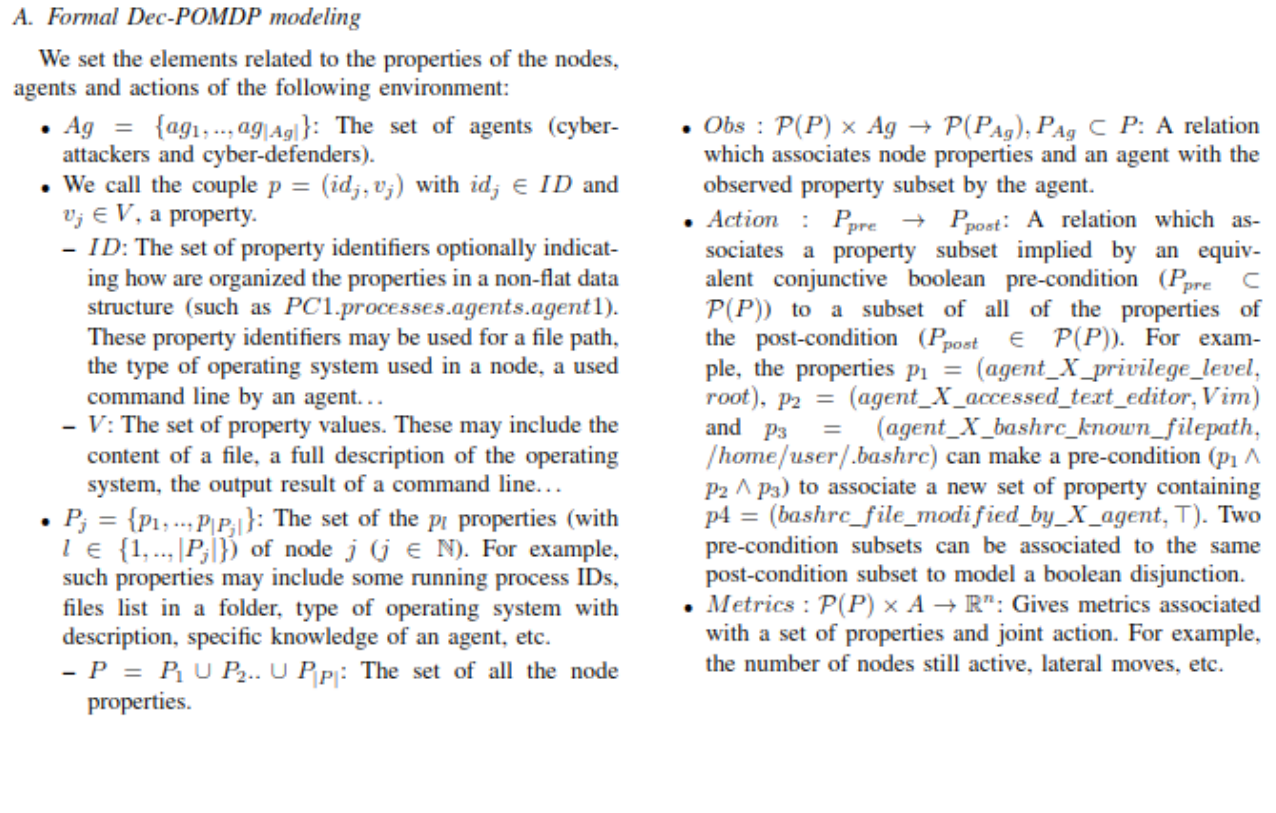
\includegraphics[scale=0.3]{figures/formal_description_1.png}
            \end{figure}

        \end{frame}

        \begin{frame}{Annexes: Dec-POMDP formal model}
            {Formal model description}

            \begin{figure}
                \centering
                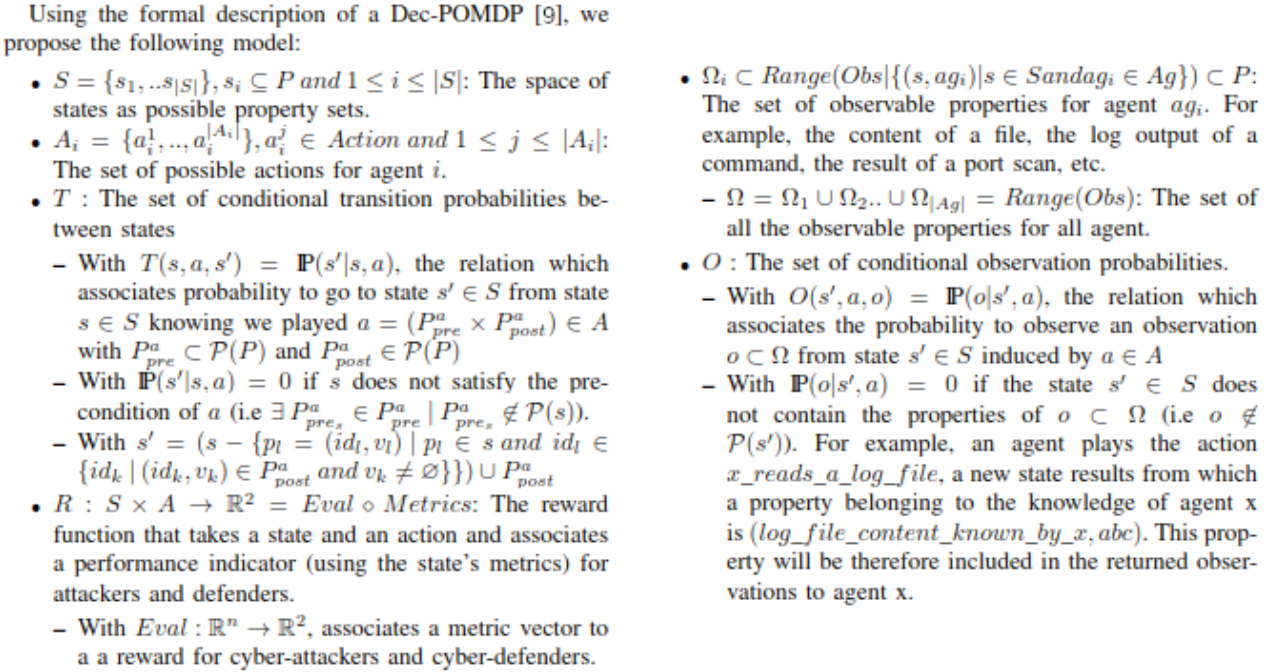
\includegraphics[scale=0.3]{figures/formal_description_2.png}
            \end{figure}

        \end{frame}
    
        
        \subsection{Attack/Defense scenarios integration}
	
        \begin{frame}{Annexes: Attack/defense scenario integration}
            {Integration approach}

            A high-level manual approach to integrate MITRE ATT\&CK information as an AD tree to formalize actions to be played in a scenario through the simulator.

            \begin{enumerate}
            
                \item Identify relevant tactics and techniques and procedures from MITRE ATT\&CK for an Advanced Persistent Threat (APT);
                
                \item Link tactics together and associated techniques, sub-techniques and procedures to create a scenario that describes how the APT group could attack the networked system;
            
                \item Establish an AD tree with tactics as top action goals while techniques, sub-techniques and procedures are in the lower part of the tree;
            
                \item Decorate the attack nodes with the MITRE ATT\&CK detection and mitigations.
                
            \end{enumerate}

        \end{frame}



        \subsection{Experimental setup}
        
	\begin{frame}{Annexes: Experimental setup}
		{Network topology}

        Based on GALLIUM APT tactics we proposed a small company like networked environment:
        \begin{itemize}
            \item The cyber-attacker agents are initially deployed on At1 and At2 and the cyber-defender agents are deployed on WS and DB.
            \item The ultimate attackers' goals is to get data from the DB server and installing one spyware on the printer server PS.
        \end{itemize}

        \begin{figure}
            \centering
            \includesvg[width=0.65\linewidth]{figures/topology.svg}
            \caption{Proposed small-scale company network topology}
            \label{fig:scenario_network_topology}
        \end{figure}
 
	\end{frame}


	\begin{frame}{Annexes: Experimental setup}
		{Attack/defense scenario}

        \vspace{-0.15cm}

        \begin{figure}
            \centering
            \includesvg[width=0.45\linewidth]{figures/ADTree.svg}

            \vspace{-0.2cm}
            
            \caption{An overview of the proposed attack/defense AD Tree}
            \label{fig:ADTree}
        \end{figure}
 
	\end{frame}


	\begin{frame}{Annexes: Experimental setup}
		{Agent behavior implementation}

            \begin{block}{Random approach}
                \begin{itemize}
                    \item The agents only choose their actions by exploring the whole action space without any criteria until reaching the goal
                    \item Allows getting a benchmark of unexpected edge failure cases and to compare with other types of agent.
                \end{itemize}
            \end{block}

            \begin{block}{Decision Tree (DT) approach}
                Reference when cyber-attackers or cyber-defenders already know the best action to take as the role of each agent is defined by a DT.
            \end{block}

            \begin{block}{Multi-Agent Reinforcement Learning (MARL) approach}
                Q-Learning~\cite{CWatkins1992} with curriculum learning for first the attackers learn how to attack before adding defenders.
            \end{block}
 
	\end{frame}